%%START SLIDE 
% 
% Copyright 2017 United States Government as represented by the
% Administrator of the National Aeronautics and Space Administration.
% All Rights Reserved.
% 
% NASA acknowledges the SETI Institute's primary role in authoring and
% producing the Kepler Data Processing Pipeline under Cooperative
% Agreement Nos. NNA04CC63A, NNX07AD96A, NNX07AD98A, NNX11AI13A,
% NNX11AI14A, NNX13AD01A & NNX13AD16A.
% 
% This file is available under the terms of the NASA Open Source Agreement
% (NOSA). You should have received a copy of this agreement with the
% Kepler source code; see the file NASA-OPEN-SOURCE-AGREEMENT.doc.
% 
% No Warranty: THE SUBJECT SOFTWARE IS PROVIDED "AS IS" WITHOUT ANY
% WARRANTY OF ANY KIND, EITHER EXPRESSED, IMPLIED, OR STATUTORY,
% INCLUDING, BUT NOT LIMITED TO, ANY WARRANTY THAT THE SUBJECT SOFTWARE
% WILL CONFORM TO SPECIFICATIONS, ANY IMPLIED WARRANTIES OF
% MERCHANTABILITY, FITNESS FOR A PARTICULAR PURPOSE, OR FREEDOM FROM
% INFRINGEMENT, ANY WARRANTY THAT THE SUBJECT SOFTWARE WILL BE ERROR
% FREE, OR ANY WARRANTY THAT DOCUMENTATION, IF PROVIDED, WILL CONFORM
% TO THE SUBJECT SOFTWARE. THIS AGREEMENT DOES NOT, IN ANY MANNER,
% CONSTITUTE AN ENDORSEMENT BY GOVERNMENT AGENCY OR ANY PRIOR RECIPIENT
% OF ANY RESULTS, RESULTING DESIGNS, HARDWARE, SOFTWARE PRODUCTS OR ANY
% OTHER APPLICATIONS RESULTING FROM USE OF THE SUBJECT SOFTWARE.
% FURTHER, GOVERNMENT AGENCY DISCLAIMS ALL WARRANTIES AND LIABILITIES
% REGARDING THIRD-PARTY SOFTWARE, IF PRESENT IN THE ORIGINAL SOFTWARE,
% AND DISTRIBUTES IT "AS IS."
% 
% Waiver and Indemnity: RECIPIENT AGREES TO WAIVE ANY AND ALL CLAIMS
% AGAINST THE UNITED STATES GOVERNMENT, ITS CONTRACTORS AND
% SUBCONTRACTORS, AS WELL AS ANY PRIOR RECIPIENT. IF RECIPIENT'S USE OF
% THE SUBJECT SOFTWARE RESULTS IN ANY LIABILITIES, DEMANDS, DAMAGES,
% EXPENSES OR LOSSES ARISING FROM SUCH USE, INCLUDING ANY DAMAGES FROM
% PRODUCTS BASED ON, OR RESULTING FROM, RECIPIENT'S USE OF THE SUBJECT
% SOFTWARE, RECIPIENT SHALL INDEMNIFY AND HOLD HARMLESS THE UNITED
% STATES GOVERNMENT, ITS CONTRACTORS AND SUBCONTRACTORS, AS WELL AS ANY
% PRIOR RECIPIENT, TO THE EXTENT PERMITTED BY LAW. RECIPIENT'S SOLE
% REMEDY FOR ANY SUCH MATTER SHALL BE THE IMMEDIATE, UNILATERAL
% TERMINATION OF THIS AGREEMENT.
%
\cleardoublepage

\renewcommand{\slideTitle}{{\Huge {\bf Collateral Data (All Chs)}}}
%
% Copyright 2017 United States Government as represented by the
% Administrator of the National Aeronautics and Space Administration.
% All Rights Reserved.
% 
% This file is available under the terms of the NASA Open Source Agreement
% (NOSA). You should have received a copy of this agreement with the
% Kepler source code; see the file NASA-OPEN-SOURCE-AGREEMENT.doc.
% 
% No Warranty: THE SUBJECT SOFTWARE IS PROVIDED "AS IS" WITHOUT ANY
% WARRANTY OF ANY KIND, EITHER EXPRESSED, IMPLIED, OR STATUTORY,
% INCLUDING, BUT NOT LIMITED TO, ANY WARRANTY THAT THE SUBJECT SOFTWARE
% WILL CONFORM TO SPECIFICATIONS, ANY IMPLIED WARRANTIES OF
% MERCHANTABILITY, FITNESS FOR A PARTICULAR PURPOSE, OR FREEDOM FROM
% INFRINGEMENT, ANY WARRANTY THAT THE SUBJECT SOFTWARE WILL BE ERROR
% FREE, OR ANY WARRANTY THAT DOCUMENTATION, IF PROVIDED, WILL CONFORM
% TO THE SUBJECT SOFTWARE. THIS AGREEMENT DOES NOT, IN ANY MANNER,
% CONSTITUTE AN ENDORSEMENT BY GOVERNMENT AGENCY OR ANY PRIOR RECIPIENT
% OF ANY RESULTS, RESULTING DESIGNS, HARDWARE, SOFTWARE PRODUCTS OR ANY
% OTHER APPLICATIONS RESULTING FROM USE OF THE SUBJECT SOFTWARE.
% FURTHER, GOVERNMENT AGENCY DISCLAIMS ALL WARRANTIES AND LIABILITIES
% REGARDING THIRD-PARTY SOFTWARE, IF PRESENT IN THE ORIGINAL SOFTWARE,
% AND DISTRIBUTES IT "AS IS."
%
% Waiver and Indemnity: RECIPIENT AGREES TO WAIVE ANY AND ALL CLAIMS
% AGAINST THE UNITED STATES GOVERNMENT, ITS CONTRACTORS AND
% SUBCONTRACTORS, AS WELL AS ANY PRIOR RECIPIENT. IF RECIPIENT'S USE OF
% THE SUBJECT SOFTWARE RESULTS IN ANY LIABILITIES, DEMANDS, DAMAGES,
% EXPENSES OR LOSSES ARISING FROM SUCH USE, INCLUDING ANY DAMAGES FROM
% PRODUCTS BASED ON, OR RESULTING FROM, RECIPIENT'S USE OF THE SUBJECT
% SOFTWARE, RECIPIENT SHALL INDEMNIFY AND HOLD HARMLESS THE UNITED
% STATES GOVERNMENT, ITS CONTRACTORS AND SUBCONTRACTORS, AS WELL AS ANY
% PRIOR RECIPIENT, TO THE EXTENT PERMITTED BY LAW. RECIPIENT'S SOLE
% REMEDY FOR ANY SUCH MATTER SHALL BE THE IMMEDIATE, UNILATERAL
% TERMINATION OF THIS AGREEMENT.
%
\cleardoublepage
\begin{figure*}[h!]
  \centering
  \subfigure{\includegraphics[width=1in]{\logo}}
  \hfill
  \slideTitle
  \hfill
  \subfigure{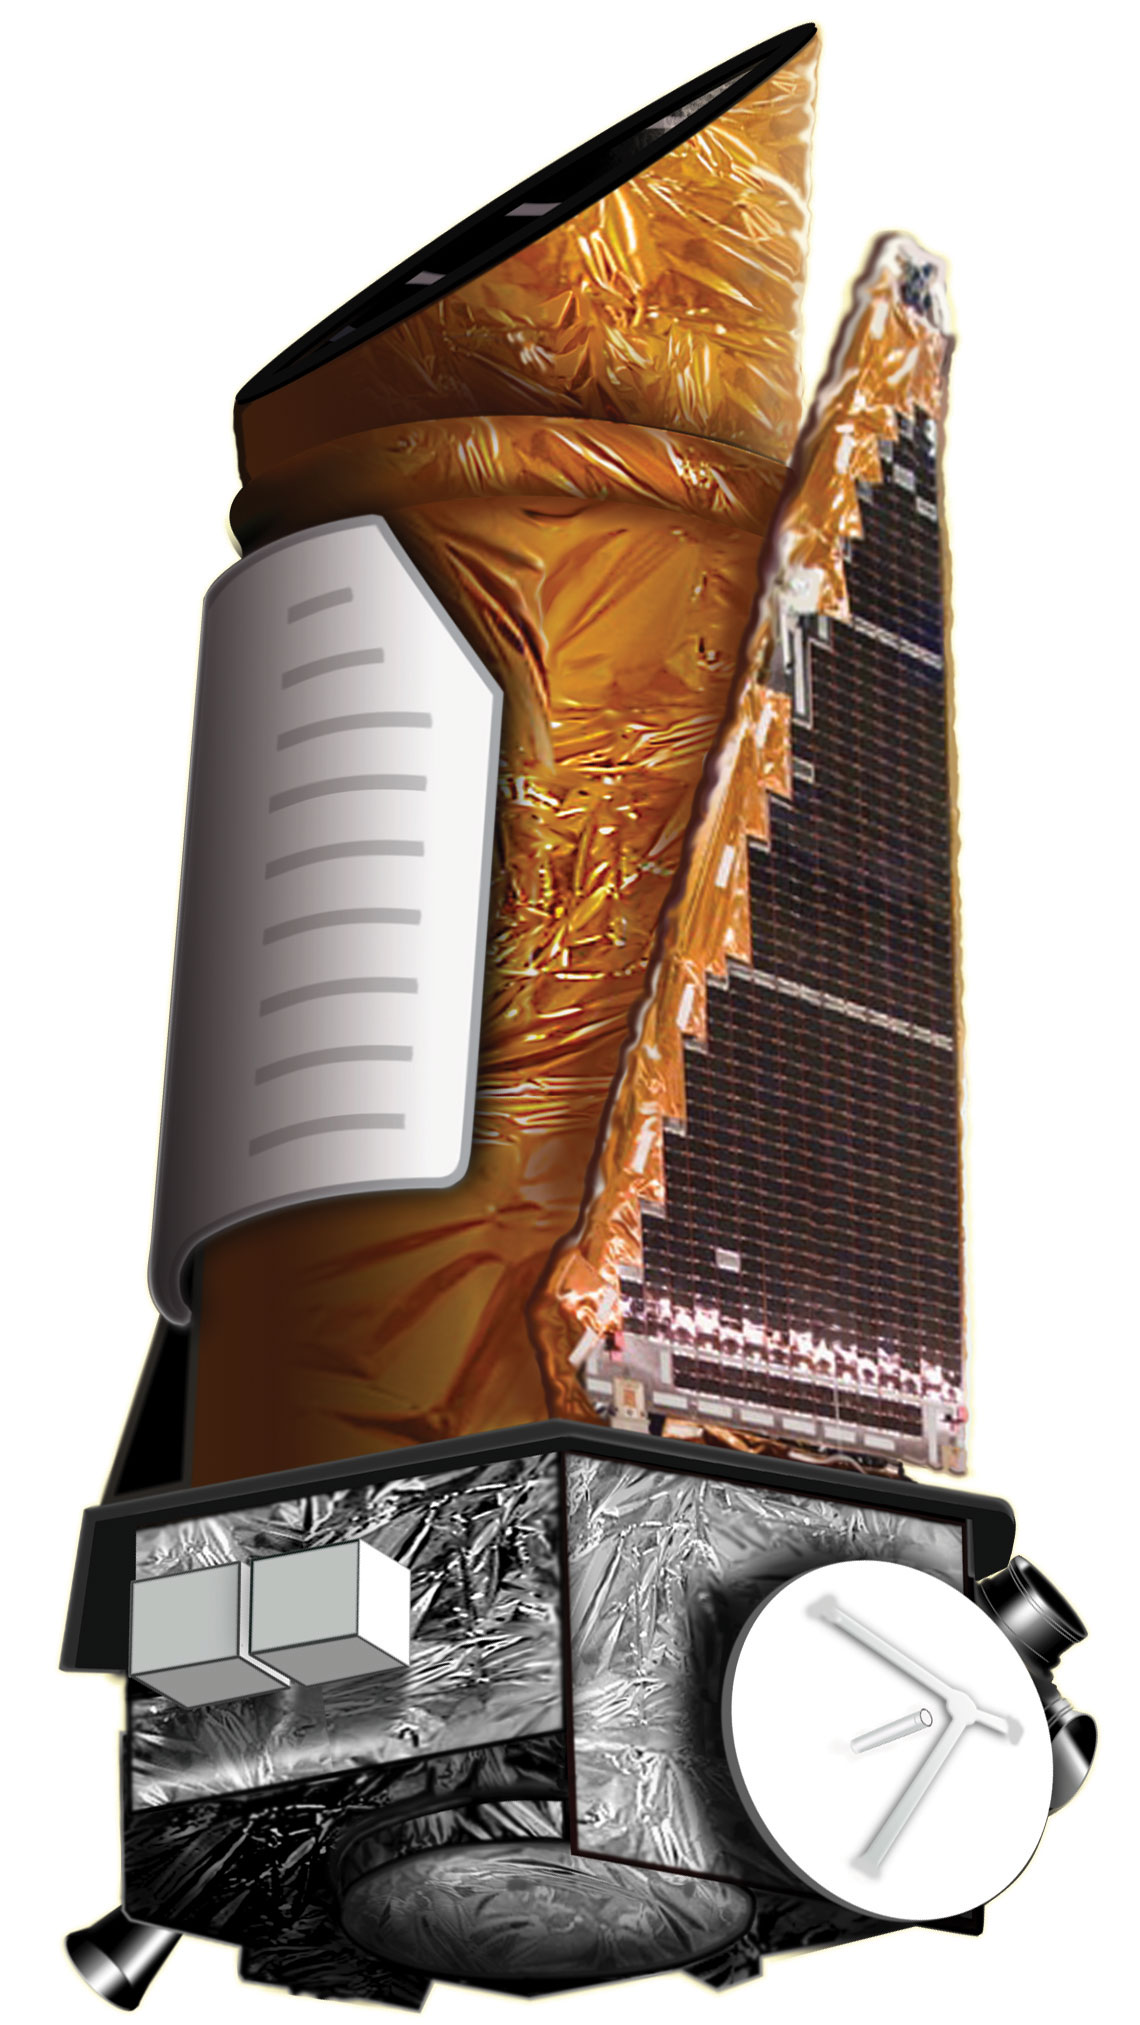
\includegraphics[angle=45,width=1in]{Kepler_spacecraft.png}}
\end{figure*}
\hrule


\begin{figure*}[h!]
  \centering
  \includegraphics[width=0.45\textwidth]{\BlackResidualsPerRowPerChannel}
  \caption{Median black residuals per row per channel}
\end{figure*}

%% END SLIDE 


%%START SLIDE 
\cleardoublepage

\renewcommand{\slideTitle}{{\Huge {\bf \quarter\ Median Masked Smear (All Chs)}}}
%
% Copyright 2017 United States Government as represented by the
% Administrator of the National Aeronautics and Space Administration.
% All Rights Reserved.
% 
% This file is available under the terms of the NASA Open Source Agreement
% (NOSA). You should have received a copy of this agreement with the
% Kepler source code; see the file NASA-OPEN-SOURCE-AGREEMENT.doc.
% 
% No Warranty: THE SUBJECT SOFTWARE IS PROVIDED "AS IS" WITHOUT ANY
% WARRANTY OF ANY KIND, EITHER EXPRESSED, IMPLIED, OR STATUTORY,
% INCLUDING, BUT NOT LIMITED TO, ANY WARRANTY THAT THE SUBJECT SOFTWARE
% WILL CONFORM TO SPECIFICATIONS, ANY IMPLIED WARRANTIES OF
% MERCHANTABILITY, FITNESS FOR A PARTICULAR PURPOSE, OR FREEDOM FROM
% INFRINGEMENT, ANY WARRANTY THAT THE SUBJECT SOFTWARE WILL BE ERROR
% FREE, OR ANY WARRANTY THAT DOCUMENTATION, IF PROVIDED, WILL CONFORM
% TO THE SUBJECT SOFTWARE. THIS AGREEMENT DOES NOT, IN ANY MANNER,
% CONSTITUTE AN ENDORSEMENT BY GOVERNMENT AGENCY OR ANY PRIOR RECIPIENT
% OF ANY RESULTS, RESULTING DESIGNS, HARDWARE, SOFTWARE PRODUCTS OR ANY
% OTHER APPLICATIONS RESULTING FROM USE OF THE SUBJECT SOFTWARE.
% FURTHER, GOVERNMENT AGENCY DISCLAIMS ALL WARRANTIES AND LIABILITIES
% REGARDING THIRD-PARTY SOFTWARE, IF PRESENT IN THE ORIGINAL SOFTWARE,
% AND DISTRIBUTES IT "AS IS."
%
% Waiver and Indemnity: RECIPIENT AGREES TO WAIVE ANY AND ALL CLAIMS
% AGAINST THE UNITED STATES GOVERNMENT, ITS CONTRACTORS AND
% SUBCONTRACTORS, AS WELL AS ANY PRIOR RECIPIENT. IF RECIPIENT'S USE OF
% THE SUBJECT SOFTWARE RESULTS IN ANY LIABILITIES, DEMANDS, DAMAGES,
% EXPENSES OR LOSSES ARISING FROM SUCH USE, INCLUDING ANY DAMAGES FROM
% PRODUCTS BASED ON, OR RESULTING FROM, RECIPIENT'S USE OF THE SUBJECT
% SOFTWARE, RECIPIENT SHALL INDEMNIFY AND HOLD HARMLESS THE UNITED
% STATES GOVERNMENT, ITS CONTRACTORS AND SUBCONTRACTORS, AS WELL AS ANY
% PRIOR RECIPIENT, TO THE EXTENT PERMITTED BY LAW. RECIPIENT'S SOLE
% REMEDY FOR ANY SUCH MATTER SHALL BE THE IMMEDIATE, UNILATERAL
% TERMINATION OF THIS AGREEMENT.
%
\cleardoublepage
\begin{figure*}[h!]
  \centering
  \subfigure{\includegraphics[width=1in]{\logo}}
  \hfill
  \slideTitle
  \hfill
  \subfigure{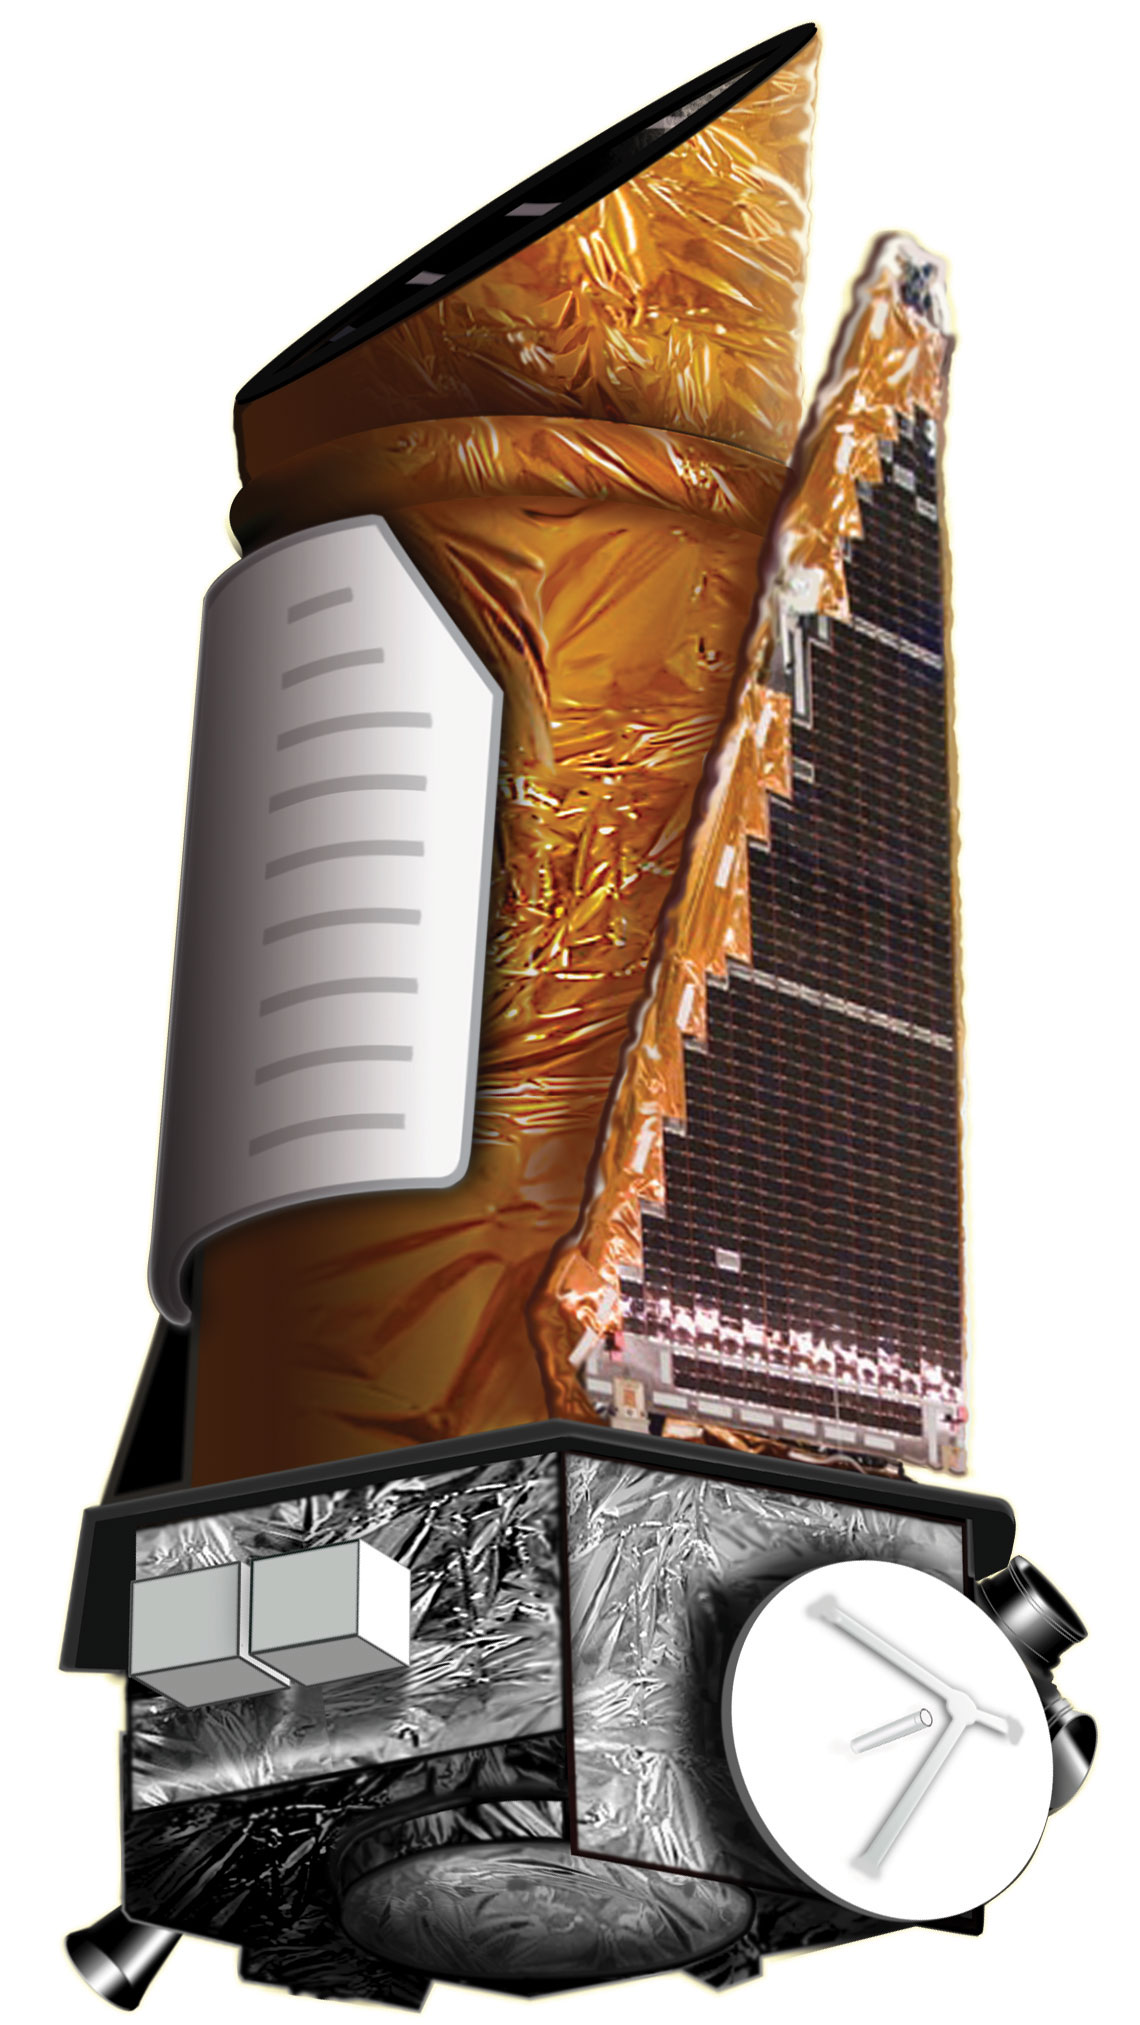
\includegraphics[angle=45,width=1in]{Kepler_spacecraft.png}}
\end{figure*}
\hrule


\begin{figure*}[h!]
  \centering
  \subfigure[Median masked smear pixels per col per channel]{\includegraphics[width=0.45\textwidth]{\MaskedSmearPerColPerChannel}}
  \subfigure[Median masked smear pixels per cad per channel]{\includegraphics[width=0.45\textwidth]{\MaskedSmearPerCadPerChannel}}
\end{figure*}

%% END SLIDE 


%%START SLIDE 
\cleardoublepage

\renewcommand{\slideTitle}{{\Huge {\bf \quarter\ Median Virtual Smear (All Chs)}}}
%
% Copyright 2017 United States Government as represented by the
% Administrator of the National Aeronautics and Space Administration.
% All Rights Reserved.
% 
% This file is available under the terms of the NASA Open Source Agreement
% (NOSA). You should have received a copy of this agreement with the
% Kepler source code; see the file NASA-OPEN-SOURCE-AGREEMENT.doc.
% 
% No Warranty: THE SUBJECT SOFTWARE IS PROVIDED "AS IS" WITHOUT ANY
% WARRANTY OF ANY KIND, EITHER EXPRESSED, IMPLIED, OR STATUTORY,
% INCLUDING, BUT NOT LIMITED TO, ANY WARRANTY THAT THE SUBJECT SOFTWARE
% WILL CONFORM TO SPECIFICATIONS, ANY IMPLIED WARRANTIES OF
% MERCHANTABILITY, FITNESS FOR A PARTICULAR PURPOSE, OR FREEDOM FROM
% INFRINGEMENT, ANY WARRANTY THAT THE SUBJECT SOFTWARE WILL BE ERROR
% FREE, OR ANY WARRANTY THAT DOCUMENTATION, IF PROVIDED, WILL CONFORM
% TO THE SUBJECT SOFTWARE. THIS AGREEMENT DOES NOT, IN ANY MANNER,
% CONSTITUTE AN ENDORSEMENT BY GOVERNMENT AGENCY OR ANY PRIOR RECIPIENT
% OF ANY RESULTS, RESULTING DESIGNS, HARDWARE, SOFTWARE PRODUCTS OR ANY
% OTHER APPLICATIONS RESULTING FROM USE OF THE SUBJECT SOFTWARE.
% FURTHER, GOVERNMENT AGENCY DISCLAIMS ALL WARRANTIES AND LIABILITIES
% REGARDING THIRD-PARTY SOFTWARE, IF PRESENT IN THE ORIGINAL SOFTWARE,
% AND DISTRIBUTES IT "AS IS."
%
% Waiver and Indemnity: RECIPIENT AGREES TO WAIVE ANY AND ALL CLAIMS
% AGAINST THE UNITED STATES GOVERNMENT, ITS CONTRACTORS AND
% SUBCONTRACTORS, AS WELL AS ANY PRIOR RECIPIENT. IF RECIPIENT'S USE OF
% THE SUBJECT SOFTWARE RESULTS IN ANY LIABILITIES, DEMANDS, DAMAGES,
% EXPENSES OR LOSSES ARISING FROM SUCH USE, INCLUDING ANY DAMAGES FROM
% PRODUCTS BASED ON, OR RESULTING FROM, RECIPIENT'S USE OF THE SUBJECT
% SOFTWARE, RECIPIENT SHALL INDEMNIFY AND HOLD HARMLESS THE UNITED
% STATES GOVERNMENT, ITS CONTRACTORS AND SUBCONTRACTORS, AS WELL AS ANY
% PRIOR RECIPIENT, TO THE EXTENT PERMITTED BY LAW. RECIPIENT'S SOLE
% REMEDY FOR ANY SUCH MATTER SHALL BE THE IMMEDIATE, UNILATERAL
% TERMINATION OF THIS AGREEMENT.
%
\cleardoublepage
\begin{figure*}[h!]
  \centering
  \subfigure{\includegraphics[width=1in]{\logo}}
  \hfill
  \slideTitle
  \hfill
  \subfigure{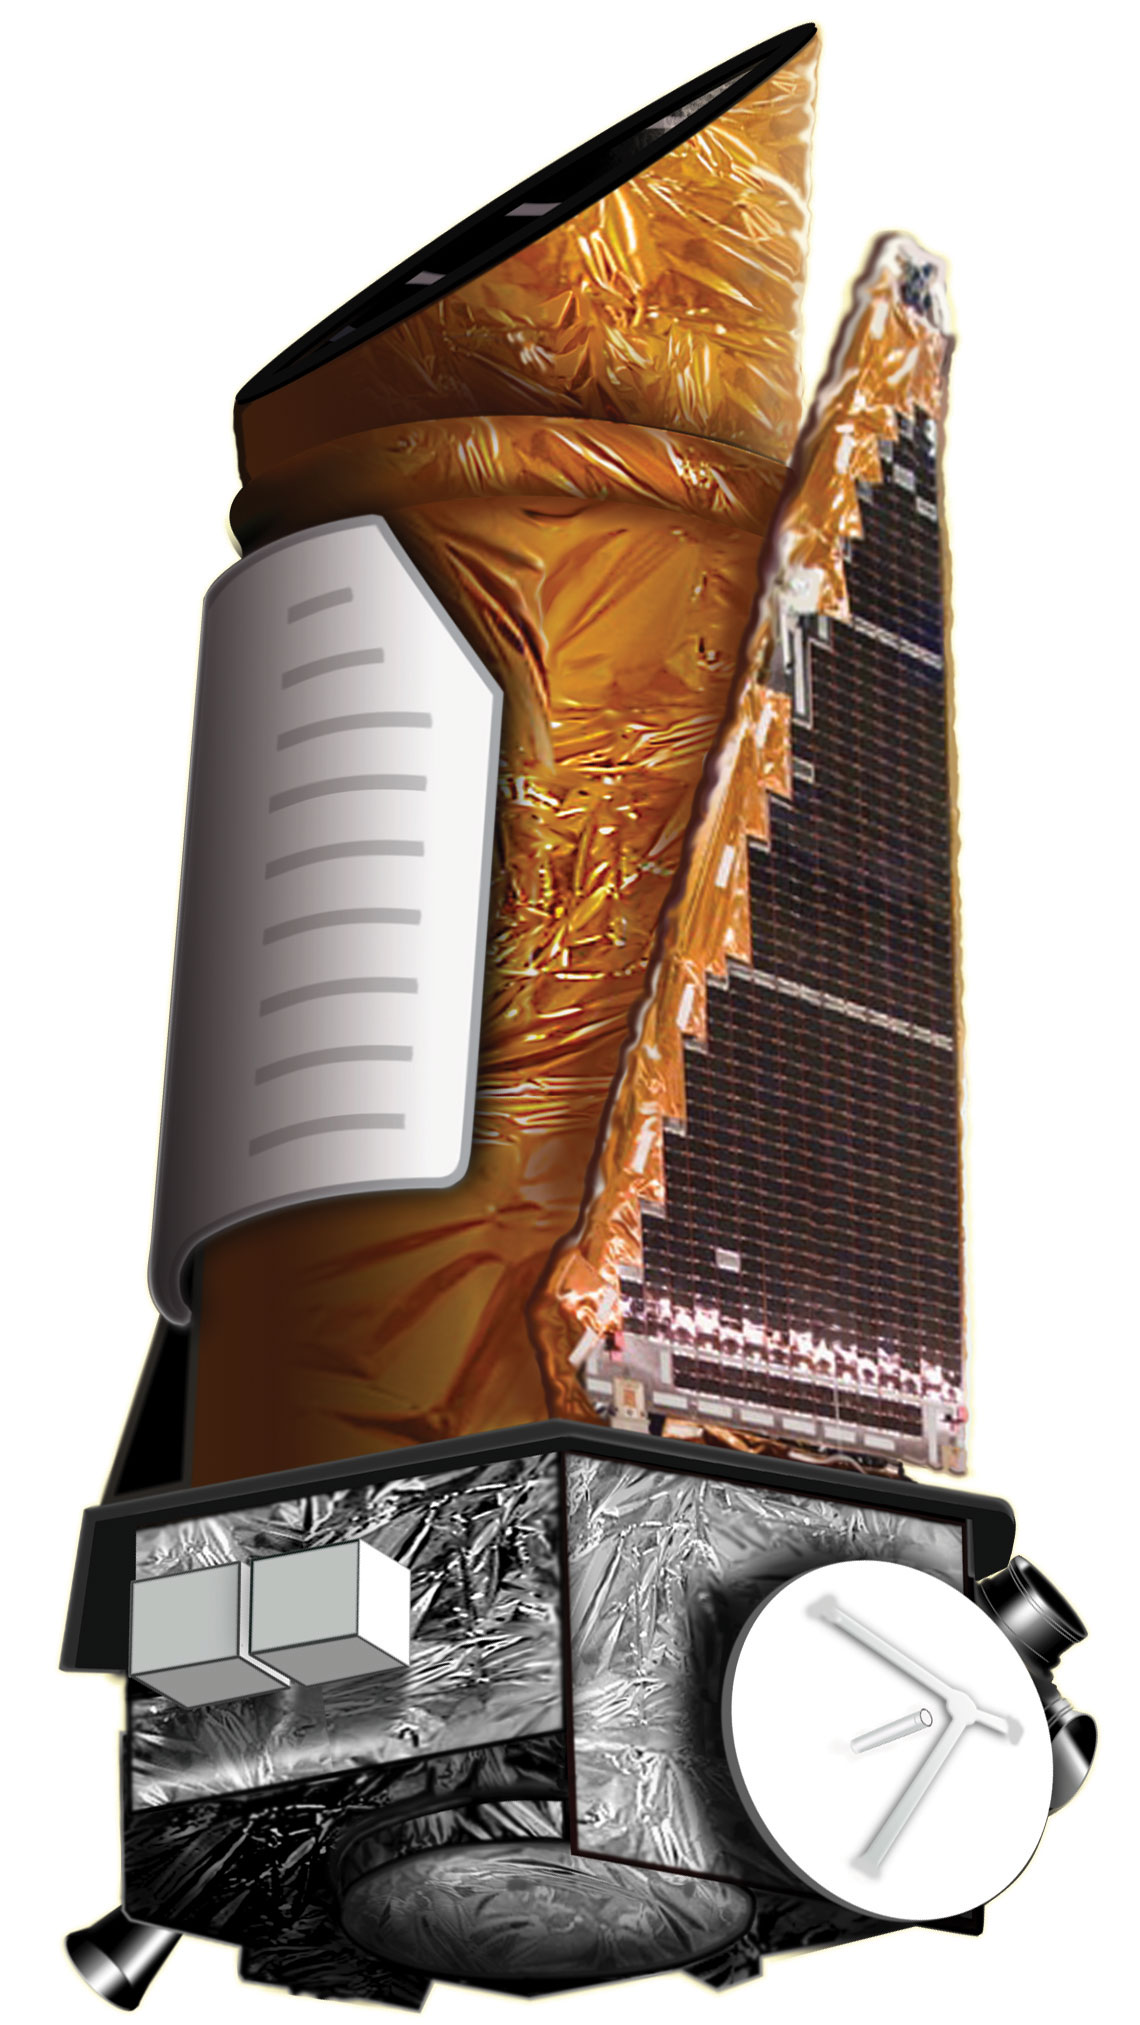
\includegraphics[angle=45,width=1in]{Kepler_spacecraft.png}}
\end{figure*}
\hrule


\begin{figure*}[h!]
  \centering
  \subfigure[Median virtual smear pixels per col per channel]{\includegraphics[width=0.45\textwidth]{\VirtualSmearPerColPerChannel}}
  \subfigure[Median virtual smear pixels per cad per channel]{\includegraphics[width=0.45\textwidth]{\VirtualSmearPerCadPerChannel}}
\end{figure*}

%% END SLIDE 


%%START SLIDE 
\cleardoublepage

\renewcommand{\slideTitle}{\Huge {\bf \quarter\ Median (Masked-Virtual) Smear (All Chs)}}
%
% Copyright 2017 United States Government as represented by the
% Administrator of the National Aeronautics and Space Administration.
% All Rights Reserved.
% 
% This file is available under the terms of the NASA Open Source Agreement
% (NOSA). You should have received a copy of this agreement with the
% Kepler source code; see the file NASA-OPEN-SOURCE-AGREEMENT.doc.
% 
% No Warranty: THE SUBJECT SOFTWARE IS PROVIDED "AS IS" WITHOUT ANY
% WARRANTY OF ANY KIND, EITHER EXPRESSED, IMPLIED, OR STATUTORY,
% INCLUDING, BUT NOT LIMITED TO, ANY WARRANTY THAT THE SUBJECT SOFTWARE
% WILL CONFORM TO SPECIFICATIONS, ANY IMPLIED WARRANTIES OF
% MERCHANTABILITY, FITNESS FOR A PARTICULAR PURPOSE, OR FREEDOM FROM
% INFRINGEMENT, ANY WARRANTY THAT THE SUBJECT SOFTWARE WILL BE ERROR
% FREE, OR ANY WARRANTY THAT DOCUMENTATION, IF PROVIDED, WILL CONFORM
% TO THE SUBJECT SOFTWARE. THIS AGREEMENT DOES NOT, IN ANY MANNER,
% CONSTITUTE AN ENDORSEMENT BY GOVERNMENT AGENCY OR ANY PRIOR RECIPIENT
% OF ANY RESULTS, RESULTING DESIGNS, HARDWARE, SOFTWARE PRODUCTS OR ANY
% OTHER APPLICATIONS RESULTING FROM USE OF THE SUBJECT SOFTWARE.
% FURTHER, GOVERNMENT AGENCY DISCLAIMS ALL WARRANTIES AND LIABILITIES
% REGARDING THIRD-PARTY SOFTWARE, IF PRESENT IN THE ORIGINAL SOFTWARE,
% AND DISTRIBUTES IT "AS IS."
%
% Waiver and Indemnity: RECIPIENT AGREES TO WAIVE ANY AND ALL CLAIMS
% AGAINST THE UNITED STATES GOVERNMENT, ITS CONTRACTORS AND
% SUBCONTRACTORS, AS WELL AS ANY PRIOR RECIPIENT. IF RECIPIENT'S USE OF
% THE SUBJECT SOFTWARE RESULTS IN ANY LIABILITIES, DEMANDS, DAMAGES,
% EXPENSES OR LOSSES ARISING FROM SUCH USE, INCLUDING ANY DAMAGES FROM
% PRODUCTS BASED ON, OR RESULTING FROM, RECIPIENT'S USE OF THE SUBJECT
% SOFTWARE, RECIPIENT SHALL INDEMNIFY AND HOLD HARMLESS THE UNITED
% STATES GOVERNMENT, ITS CONTRACTORS AND SUBCONTRACTORS, AS WELL AS ANY
% PRIOR RECIPIENT, TO THE EXTENT PERMITTED BY LAW. RECIPIENT'S SOLE
% REMEDY FOR ANY SUCH MATTER SHALL BE THE IMMEDIATE, UNILATERAL
% TERMINATION OF THIS AGREEMENT.
%
\cleardoublepage
\begin{figure*}[h!]
  \centering
  \subfigure{\includegraphics[width=1in]{\logo}}
  \hfill
  \slideTitle
  \hfill
  \subfigure{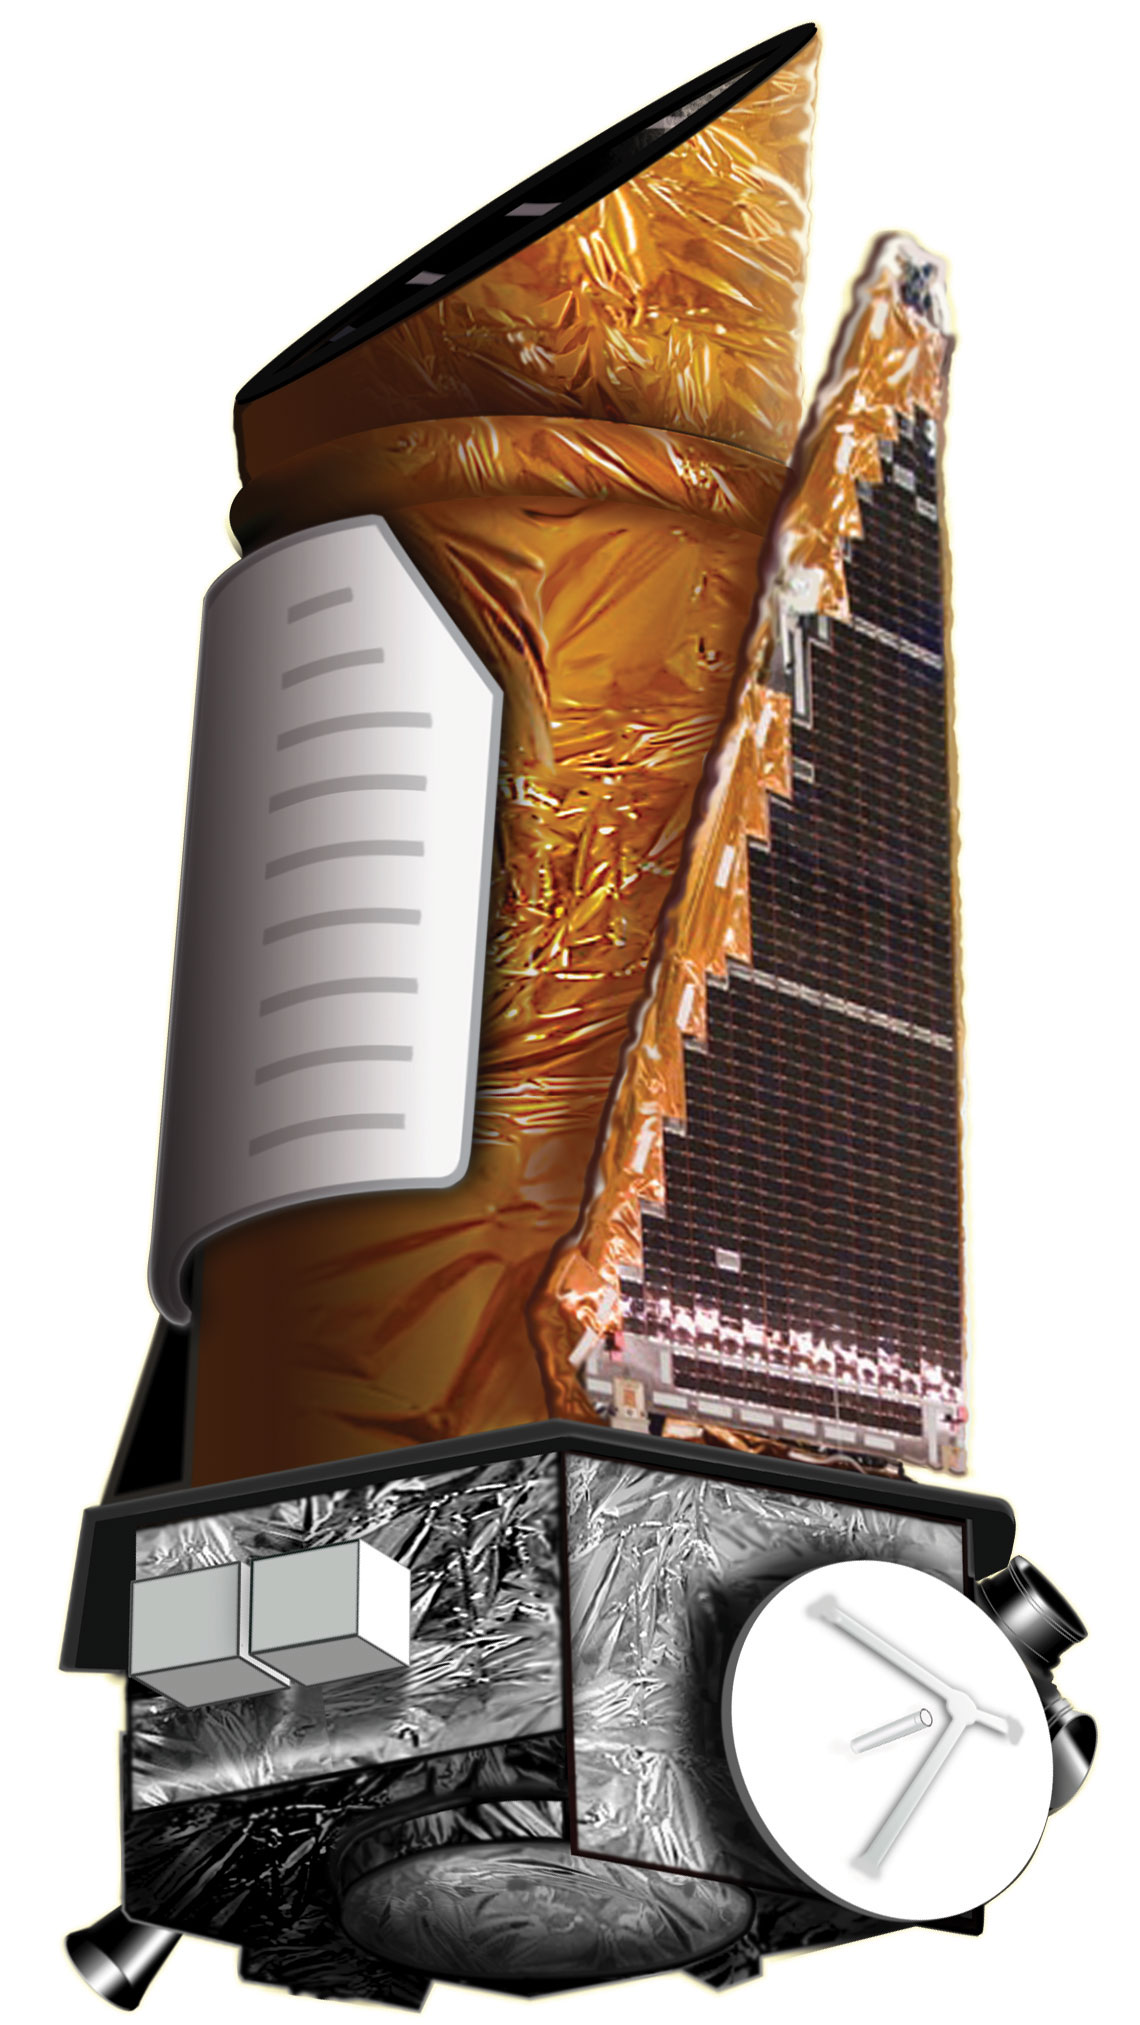
\includegraphics[angle=45,width=1in]{Kepler_spacecraft.png}}
\end{figure*}
\hrule


\begin{figure*}[h!]
  \centering
  \subfigure[Median (masked-virtual) smear pixels per col per channel]{\includegraphics[width=0.45\textwidth]{\SmearDiffPerColPerChannel}}
  \subfigure[Median (masked-virtual) smear pixels per cad per channel]{\includegraphics[width=0.45\textwidth]{\SmearDiffPerCadPerChannel}}
\end{figure*}

%% END SLIDE 

